\chapter{Research Methodology and Data}

This chapter focuses on demonstrating and explaining how the model was designed and trained. An overview of the design and architecture is given. Relevant training hyperparameters are discussed. Datasets are presented and analysed. Challenges are explained together with changes and adjustments that were made during the process. Finally, goals and criteria for the expected results are defined.

To reiterate, the current problem is to find out if a Graph Neural Network (\gls{gnn}) based method can compete at solving the Maximum Weighted Matching (\gls{mwm}) problem compared to other approximation methods such as the greedy algorithm.

\section{Challenges}

It is common to think of a neural network as a black box that takes in data as input and outputs some predictions. In our case, the data is a graph consisting of vertices connected by weighted edges and the expected answer should be pairs of adjacent vertices that are matched together or, equivalently, a list of the corresponding edges.

As mentioned, the idea behind supervised learning is to give the correct answers to a model, so it can, by trial and error, learn from it. These answers are not included in the initial datasets, so the optimal solutions need to be calculated. To find the optimal solution, the Blossom algorithm implemented by Rantwijk in Python was used \cite{mwmBlossom}. This does, however, point out an important weakness of the supervised approach. Obviously, a model needs to be able to handle graphs of different sizes, and it is the large ones that are most interesting. Finding an optimal solution for algorithmic problems for the large graphs can be time-consuming. At the same time, a model needs as much data as possible to learn, leading to multiple large graphs consuming too much time during training. This poses a question of whether it is possible for the model to learn from small and medium-sized graphs that are not as time-consuming and apply the learned patterns to solve larger graphs.

Another important aspect that must be taken into consideration is that it is unlikely for the model to fully follow the restrictions of the problem. As an example, the model might decide to match the same node to two neighbors at the same time, which should not be allowed. 

\section{Main Idea}

To summarize, given a weighted undirected graph, the \gls{gnn} must predict a valid subset of non-adjacent edges that maximize the total weight. The \gls{gnn} must teke a graph as an input. The size of the input layer will be equal to the amount of features nodes have. Initially, nodes do not have any features and, in that case, all nodes can be assigned a single feature with $value = 1$. Later, however, we experiment with adding additional precomputed features. The output layer will be of size two, representing the two possible outcomes for whether each edge should be in the matching or not. 

To check that a solution is valid, instead of picking all the edges with a probability higher than 50\%, the edges can be sorted by their probabilities and greedily picked in that order as long as they don't break the validity of the solution. It might sound illogical to use a greedy algorithm on the models' output to beat the normal greedy algorithm with weights, but the fact that edges are now sorted not by their weight, but a score decided by the \gls{gnn} does make a difference, since it can take multiple features in consideration when assigning probabilities. Some of these features come naturally from the structure of the graph, and some we can manually add during preprocessing. This approach does imply that the expected running time on the \gls{gnn} will be higher than that of a greedy algorithm due to the fact that the sorting of edges still remains, but on top of that, the graph must be processed by the model.

\gls{nn}s have several hyperparameters and methods that can be tuned to make a model better suited for the task. With unlimited resources and time, one could search for the best combination of the hyperparameters by trying as many combinations as possible and training a separate model for each combination. Then choose the one with the best performance. However, this is a time-consuming procedure, therefore, in the current work, the exploration of hyperparameters has been narrowed down to the ones that seemed most important and indicated a positive impact during early experiments. For training, Adam optimizer was used \cite{kingma2017adam}. The optimizer is used to adjust the weights of the network during training. Adam optimizer has several hyperparameters that can be useful to achieve better results and is one of the commonly used optimizers.

During the experiments the following hyperparameters were tested:
\begin{itemize}
\item Epochs - the number of training iterations
\item Learning rate - by how much the weights of the model should be adjusted after each iteration
\item Network depth - amount of layers 
\item Network width - neurons in the layers
\item Class weights - how much should the model focus on a given class. Classes being: 
	\begin{itemize}
	\item 0 = is NOT in the solution.
	\item 1 = is in the solution.
	\end{itemize}	
\item Weight decay - used to keep \gls{gnn} weight values relatively small and decrease chances of the overfitting. 

\item Additionally other methods were tried such as augmenting data (adding extra features to the nodes during preproccessing): 
	\begin{itemize}
	\item Degree - how many neighbours a node has
	\item Weight relative to the sum of neighbours.
	\item Weight difference from the sum of the neighbours.
	\item Sum of the weights. 
	\item 1st largest weight, 2nd largest weight.
	\end{itemize}

\item Aggregation function - for the features of the neighbouring nodes 
\end{itemize}

Experimenting with the hyperparameters allows one to find the configuration for the model that balances it between overgeneralizing its prediction and memorizing the training dataset without being able to make accurate predictions based on the unseen data. Low learning rates make the training process more time-consuming, while large learning rates make weight adjustments that can overstep weight values that potentially could have improved performance. The depth and the width of the network are responsible for the level of complexity the model can learn. However, one does not need an overly complex model, since it both slows the model down and makes it susceptible to memorizing the dataset. Class weights can help with the distribution of data. If nodes in a graph have multiple neighbours, a good portion of the edges will not be in the solution. The model might be affected by the dominant number of edges that are not part of the solution to the point where it is not focusing enough on finding the ones that are in the solution. Adding extra features might help the model to find new patterns. The aggregation function is the only parameter specific to the \gls{gnn} and is responsible for the gathering of information about the neighboring nodes.

\section{Data}
\label{sec:dataanalysis}
The model should be capable of solving any graph relevant to the \gls{mwm} problem. For a graph to be relevant for the task, it is only required to be undirected and have weighted edges. Although one can also use unweighted graphs with all edge weights set to one.

For training and experimenting with the \gls{gnn}, the MNIST dataset was used \cite{dwivedi2022benchmarking}. The dataset consists of 70000 relatively small graphs with 70 nodes and 564 edges on average. Graphs also include features for the edges representing distances between nodes. These features are used as the weights for the problem. Although the graphs in this dataset are relatively small, they have some fitting qualities, such as nodes having multiple neighbors, creating more possible ways to match the nodes. The small size also makes it less time-consuming to train the models and try different approaches, as well as to show whether a \gls{gnn} trained on smaller graphs can transfer its knowledge to larger graphs.

Training and testing the model only on MNIST graphs does not cover all the various graphs that can occur. Therefore, the model had to be tested on other graphs that have different structures and weight distributions. Models trained exclusively on the MNIST dataset did not perform as well on other graphs as one might have expected. Therefore, another dataset was made to cover a larger variety of graphs. The dataset was a collection of random graphs from SuiteSparse database that ranged between 100 and 10000 nodes. As described in more detail in the \hyperref[sec:preprocessing]{3.4.4 Data preprocessing section}, some of the graphs did not have edge weights. In these cases, random weights were generated. The graphs were collected by using the following filter in Python that downloads a list of the graphs that fit the set criteria:

\begin{lstlisting}[language=Python,caption{Filter used to find graphs from different datasets}]
import ssgetpy as ss
dataset = ss.search( 
		limit = 10000,
		kind='Weighted',
		rowbounds = (50,10000),
		colbounds = (50,10000),
		nzbounds = (10,1000000))
\end{lstlisting}

Including truly large graphs in training caused problems with insufficient memory and too long training time, but the final model was still tested on the larger graphs than ones used in training. The graphs were taken from different datasets described in table \ref{large graphs for test}.

\begin{table}[h!]
\centering
\captionof{table}{Names and sizes of graphs used for testing} 
\begin{tabular}{||c | c | c||} 
\hline
 Graph & Nodes & Edges \\ [0.5ex] 
 \hline\hline
 G22 & 2 000 & 40 000 \\
 \hline
 Cage9 & 3 500 & 38 000 \\
 \hline
 California & 5 000 & 20 000 \\
 \hline
 G55 & 5 000 & 25 000 \\
 \hline
 Cage10 & 11 000 & 140 000 \\
 \hline
 as-22july06 & 22 000 & 96 000 \\
 \hline
 dictionary28 & 39 000 & 178 000 \\ [1ex] 
 \hline
\end{tabular}
\label{large graphs for test}
\end{table}

Small handcrafted graphs as well as modified versions of the existing graphs, demonstrated in the \hyperref[sec:greedybadcase]{4.3.1 Weakness of the greedy algorithm}, were used to test if \gls{gnn} can at least beat the cases specifically made to put greedy approach in a disadvantage.

\section{Architecture}
\label{sec:architecture}
During the experiments, the architecture of the \gls{gnn} model itself had mostly minor changes, but two rather different graph preprocessing steps were used. In both cases we use \gls{gcn} layers (GCNConv) \cite{gcnpaper}. The GCNConv layer fits well for the purpose of this task due to it's message passing utilizing the edge weights that are the crucial part for solving \gls{mwm}. The input layer has the same size as the number of node features. Then the graph convolutional layers are added, the depth and width of the middle layers vary depending on the temporary training results. For the output layer, a logarithmic softmax function is applied to obtain the log-probabilities required to calculate the negative log likelihood loss. These probabilities can then be translated into normal probabilities. 

The next code snippet \ref{Pytorch GCN for the line graph} shows an example of the Python implementation for the line graph \gls{gcn}. GCNConv implements a single layer of the network. The input layer is the size of the number of vertex features (5 in this example). The input layer connects to 640 neuron wide GCNConv layers. The last layer outputs predictions for each vertex through Linear layer with one neuron for each possible outcome. The first neuron represents the probability of the edge NOT being in the matching and the second represents the opposite. The “forward” method is used to define how the data flows from one layer to another. The “relu” function $f(x) = max(0,x)$ is a commonly used activation function for neural networks. The purpose of the activation function is to add non-linearity to the mode.

\begin{lstlisting}[caption={Pytorch GCN for the line graph}, label={Pytorch GCN for the line graph}, language=Python]
class MyGCN(torch.nn.Module):
    def __init__(self):
        super().__init__()
        self.conv1 = GCNConv(5, 640) # 5 features per each node, initialy 1
        self.conv2 = GCNConv(640, 640)
        self.lin = Linear(640, 2) # 2 classes 

    def forward(self, graph):        
        x, edge_index, edge_weight = graph.x, graph.edge_index, graph.edge_weight
        
        x = self.conv1(x, edge_index, edge_weight)
        x = F.relu(x)
        
        x = self.conv2(x, edge_index, edge_weight)
        x = F.relu(x)
        
        x = self.lin(x)
        return F.log_softmax(x, dim=1)    
\end{lstlisting}

We have also experimented with adding skip connections to the architecture. Skip connections are used to let information from one layer jump over some layers to reach the deeper ones. This method helps to emphasize the importance of earlier layers as their impact tends to vanish in deeper networks. Additionally, skip connections help the network to learn the identity function $f(x) = x$, which can be helpful in cases where complex patterns are not needed. The listing \ref{Skip connection example} shows how one can implement skip connection between first layer $self.conv1$ and the output layer $self.lin$

\begin{lstlisting}[caption={Skip connection example}, label={Skip connection example}, language=Python]
def forward(self, data):        
        x, edge_index = data.x, data.edge_index
        
        x = self.conv1(x, edge_index)
        identity = F.relu(x)
        
        x = self.conv2(identity, edge_index)
        x = F.relu(x)
        
        x = self.conv3(x, edge_index)
        x = F.relu(x)

        x = torch.cat((x,identity),1)
        x = self.lin(x)
        
        return F.log_softmax(x, dim=1)
\end{lstlisting}

Now, let us go through the process of a graph being matched using the \gls{gnn}.

\subsection{Model pipeline}

As mentioned earlier, one cannot fully trust the model to satisfy the restrictions of the problem. What is meant by the restrictions of the problem is the fact that every node can only be matched once. This is controlled by sorting the probabilities of the model's outputs in descending order and adding matches to the final solution one by one, skipping matches that already have matched nodes. Another potential problem can arise at the end when some of the nodes that can be matched were not matched at all by the model. There is a chance of that happening, since only matches with a high enough probability are used. As a starting point, the probability threshold is 50\% and above. Two precautions are taken to ensure nothing is left to waste. First, after the model is done, the potential remainder of the graph is fed to the model again. For a model, this would essentially be a new graph, and it may happen that the model manages to match the remainder given the new context. This process can be repeated several times and the break condition is if 0 matches were made in the last iteration. At that point, if anything is left, which hopefully is a small fraction of the initial graph, it can be solved using standard greedy or any other approximation algorithm, for that matter.

Passing the graph, and its consecutive remainders multiple times through the model can also be helpful to deal with the cases where one of the matches that was chosen may strongly affect how the rest of the solution will look like. This leads to the main weakness of the supervised approach. The optimal solution can be completely different if even one edge is picked or not picked by a mistake. This problem can be mitigated by picking one match at a time, updating the features and passing the graph through the model again, but it would be too time-consuming.

\begin{algorithm}
\caption{Model Pipeline}\label{alg:cap}

\begin{algorithmic}

\State inputGraph
\State $S = \emptyset$
\State g = preproccess(inputGraph)

\While{g.hasUnmatchNodes}

\State edgeProbabilities = model.makePrediction(g)
\State matches = greedyPickByProb(edgeProbabilities)
\State g = g.remove(matches)
\State S.add(matches)

\If{$matches == \emptyset$}
  \State matches = greedyPickByWeight(g.edgeWeights)
  \State g = g.remove(matches)
  \State S.add(matches)
\EndIf
\EndWhile
\State return S
\end{algorithmic}
\end{algorithm}

\subsection{Line Graph Approach}

The line graph approach was the first attempt at using a simple \gls{gnn}, which later turned out to be overly time-consuming for larger graphs to be worth further experiments. It did, however, give some useful insight as well as shown to be a proof of concept. The \hyperref[sec:preprocessing]{2.2 Graphs section} gives the description and an example of a line graph.

Convertion to a line graph makes the architecture of the \gls{gnn} model simpler. Instead of needing to ask a model to make predictions about whether each connected pair of nodes should be matched together, the line graph model can now output the probability of a node being in the matching directly, since the node now represents two connected nodes from the original graph. This also transforms the problem itself. From the perspective of the model, it is now trying to solve \gls{mwis}. \gls{gnn}s for \gls{mis} have been studied before. Nouranizadeh et. al.\ demonstrated a pooling method for solving \gls{mwis} \cite{DBLPjournals/corr/abs-2107-01410} so it would be reasonable to expect the model to be able to perform relatively well. 

Unfortunately, large graphs can explode in size when converted to line graphs and are too time-consuming in such cases. Consider a graph from figure \ref{linegraphbigexamplet} with a node $0$ in the center connected to three other nodes. The size of such a graph would be four nodes and three edges. In a line graph, that would result in a clique of three nodes with every node being connected all the other nodes. But if the node $0$ had 10 neighbors instead, the line graph will result in a clique of 10 nodes and $1/2 * 10 * (10-1) = 45$ edges. While the number of nodes in a line graph will always be equal to the number of edges in the original graph, the number of edges can be significantly larger. Since the running time of solving \gls{mwm} depends on the number of edges, there is a reason to try other approaches.

\begin{figure}[H]
    \centering

    \begin{minipage}[b]{0.4\textwidth}
    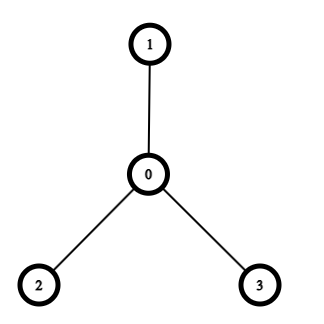
\includegraphics[width=\textwidth]{figures/linegraphbigexample}
    \caption{Original graph}
  \end{minipage}
  \hfill
  \begin{minipage}[b]{0.4\textwidth}
    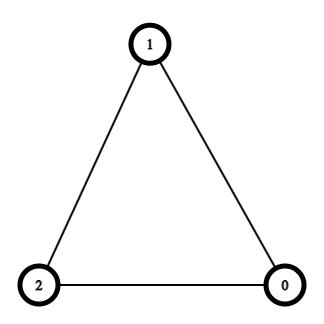
\includegraphics[width=\textwidth]{figures/linegraphnigexample2}
    \caption{Line graph}
  \end{minipage}

    \caption{Line graph convertion example }
    \label{linegraphbigexamplet}
\end{figure}

\subsection{Edge Classification Approach}

Another way of approaching this problem is to work directly on the original graphs instead of transforming them into line graphs. However, the model itself only returns some numerical representation of the nodes in the graph. To get the predictions for the edges one can add a classifier module to the existing \gls{gnn}. The purpose of this module is to predict if a pair of two nodes will be in the matching based on their embedding. The first part of the model produces embedding for each node and then, for each edge, embeddings of both nodes are put together and passed to the classifier. Finally, the model outputs probabilities of all the edges being in the matching. This approach eliminates the need for the line graph conversion which often leads to larger graphs and slower running time.

The next code snippet \ref{Pytorch GCN for the edge prediction} shows an example of the Python implementation for the edge classifier network using Pytorch libraries. The MyGCNEdge class is responsible for embedding the vertices of the graph. The input layer is the size of the number of the vertex features (5 in this example). The input layer connects to $640$ neuron wide GCNConv layers and outputs feature array of size $80$ for each vertex through Linear layer. Then EdgeClassifier class can be used to create the edge embeddings using embedEdges method that concatenates $80$ features from two endpoints of an edge together using $torch.cat()$. Each edge is then passed through an input layer with $80+80$ total features and further through fully connected Linear layers. The output layer is of size two with the logsoftmax function at the end to get the values required for the loss calculation, same as it is in the line graph model.

\begin{lstlisting}[caption={Pytorch GCN for the edge classification}, label={Pytorch GCN for the edge prediction}, language=Python]

class MyGCNEdge(torch.nn.Module):
    def __init__(self):
        super().__init__()
        self.conv1 = GCNConv(5, 640)
        self.conv2 = GCNConv(640, 640)
        self.embed = Linear(640, 80) # 80 output features per node

    def forward(self, data):        
        x, edge_index, edge_weight = data.x, data.edge_index, data.edge_weight

        x = self.conv1(x, edge_index, edge_weight)
        identity = F.relu(x)
        
        x = self.conv2(x, edge_index, edge_weight)
        x = F.relu(x)
        
        x = self.embed(x)
        return x

class EdgeClassifier(torch.nn.Module):
    def __init__(self):
        super().__init__()
        self.lin1 = Linear(160, 320) # 80 * 2 features since input is 2 nodes.
        self.lin2 = Linear(320, 2)

    def embedEdges(self, nodeEmbed, graph):
        x_src, x_dst = nodeEmbed[graph.edge_index[0]], nodeEmbed[graph.edge_index[1]]
        edgeEmbed = torch.cat([x_src, x_dst], dim=-1)        
        return edgeEmbed

    def forward(self, edgeEmbed):        
        x = self.lin1(edgeEmbed)
        x = F.relu(x)
        
        x = self.lin2(x)
        return F.log_softmax(x, dim=1)

\end{lstlisting}

\subsection{Data preprocessing}
\label{sec:preprocessing}
Not all graphs found in the database are fit for the training as is, and the ones that fit perfectly are few. Machine learning models often require some preprocessing of data before they can be used. Conversion to the line graph is one example of such a preprocessing. One might also need to augment the initial data to improve model performance. Finally, machine learning models can be vulnerable to large numerical variations in the data, such as variation of the edge weights.

For \gls{mwm}, the edge weight is the key feature that is required for the graphs to be viable. To ensure we have enough graphs to train on, and the graphs cover a variety of structures, different data source might be used. Some of the encountered graphs might lack weights and will have to receive randomly generated weights. We assign the random weights using even distribution in the range between 0 and 1. All the graphs with preexisting weights are also adjusted to be in the same range by shifting the weights to a positive range if any negative weights were detected and then dividing by the largest weight in the dataset. The weights could have been in any range, but the important thing is to have consistent weights for all the graphs. 

Another viable preprocessing step is node feature augmentation. One can use the edge weight to precompute potentialy helpfull information such as weight sum of all the edges of each node. This requires different approaches for line graph and edge prediction approaches, since in a line graph, the vertex represents an edge from the original graph.

One node feature does remain in common: the degree of the nodes or how many neighbours each node has. Although the degrees have to be calculated separately for the original and the line graph, since degree of the line graph nodes represents the number of adjacent edges of an edge in the original graph.

Line graph's node features:  

\begin{enumerate}
\item Weight relative to the sum of neighbours. For each vertex v:  \[ Wrel = v.weight  \div  (\sum_{n \in N(v)} n.weight) \]
\item Weight difference from the sum of the neighbours. For each vertex v:  \[ Wdiff = v.weight  -  (\sum_{n \in N(v)} n.weight) \]
\item Sum of the neighbouring node weights For each vertex v: \[ Wsum = (\sum_{n \in N(v)} n.weight) \]
\end{enumerate}

The motivation for adding these features is based on the idea that precalculating the relations between the edges and the neighbouring edges might allow the \gls{gcn} to find patterns easier. For example, in the line graph, if a node $n$ has weight $W(n) = 10$ and the sum of neighbouring nodes is $Wsum < 10$, then $Wrel > 1$ and any combination of two neighbouring nodes has total weight $< 10$ and therefore node $n$, that represents the edge in the original graph, should be in the solution. This is a simple case that the \gls{gnn} might find without additional features, but it serves as an example. It might be unintuitive how these features can be helpful, but one of the \gls{gnn}'s functions is to find difficult patterns, and it is worth testing such features even if their effect is not apparent. The weight of the edges is also the only input feature available in this task, so the additional features are dependent on it. 

For the original graph's node features, some adjustments are made since nodes do not have any weights assigned to them, unlike the line graph:

\begin{enumerate}
\item Sum of the weights of all the outgoing edges. For each vertex v: \[ Wsum = (\sum_{j \in N(v)} e_{v,j}.weight) \]
\item Wsum relative to the Wsum of neighbours. For each vertex v:  \[ Wrel = Wsum \div (\sum_{n \in {N(v)}} n.Wsum) \]
\item Wsum difference from the Wsum of the neighbours. For each vertex v: \[ Wdiff = Wsum - (\sum_{n \in {N(v)}} n.Wsum) \]
\end{enumerate}

\section{Result Validation}

Before looking at the results, it is important to decide how to evaluate the results properly and what is important for the problem at hand:

\begin{enumerate}
\item Time - how long an algorithm took to produce an answer. For the \gls{gnn} model, this includes model specific preprocessing such as adding additional features as well as finishing the potential remainder of the graph with a greedy algorithm.
\item Correctness - is the answer correct? In the case of \gls{mwm} the total weight acquired would be the measurement of the quality of the solution. It is unlikely that the \gls{gnn} model can find an optimal solution for more complex problems, so it is reasonable to look at how close the \gls{gnn} comes to the optimal solution.
\item Remainder - a portion of the final solutions' weight that came directly from the models' predictions. Due to the way the program is set up, if the model does not match the whole graph, the rest of the graph will need to be finished somehow. This is done by running a normal greedy algorithm at the end if anything is left. Because of that, there can be cases where the model does nothing and by default achieves 100\% result compared to what a normal greedy algorithm would. Therefore, the portion of the weights obtained directly by the model needs to be evaluated as well.
\end{enumerate}

\subsection{Sanity checks}

It might happen that during the project something goes wrong with the mode. Therefore, it is common to perform sanity checks to see if a model's inputs and outputs still make sense.

The following “sanity checks” were done:

\begin{enumerate}
\item To ensure the model and data are functioning correctly, we trained a model on a small dataset for a long time and tested it on the same data. The model should be able to memorize the provided graphs and solve the problem near perfect then.

\item Comparisons to random matchings were done. Before the training, the model has random weights and essentially will behave as if it is picking edges at random, but after some training the model is expected to start improving and perform better than a random matching would.

\item The model was tested on small handcrafted graphs that were made specifically to put the greedy algorithm at a disadvantage. If the \gls{gnn} model manages to solve such cases that indicates that the model is learning some of the patterns.
\end{enumerate}	

\section{Expected Results}

\subsection{Other observations}

One important observation was made during the analysis of the data that is worth mentioning. The difference between the optimal solution and the greedy is, in most cases, rather small. For the MNIST dataset and the majority of the graphs used from the Suite Sparse Matrix Collection, the greedy algorithm manages to reach 90+\% of the optimal weight. Assigning random evenly distributed values to the edge weights also gives the same results. For the \gls{gnn} this means that it will be rather difficult to beat the greedy algorithm since it gets fairly close to the optimal.

\subsection{Accuracy and total weight}

There exists limited amount of research specifically for for solving \gls{mwm} using \gls{gnn}. However, problems like \gls{mis} that are relatively similar to the \gls{mwm} on the line graph  can indicate that one could obtain similar results for this case as well. As discussed in the \hyperref[sec:graphneuralnetworks]{2.3 Graph Neural Networks section}, there are studies that show that \gls{gnn}s are capable of solving \gls{co} problems and beating greedy algorithms, while others indicate that improvements are still needed for it to be worth using. Therefore, it is hard to forecast any results based on previous work. It is worth noting that the greedy algorithm is relatively simple. It is conceivable that a \gls{gnn} model should be able to recognize more complex patterns that can be used to achieve better results. It is not expected for the model to be able to find an optimal solution since any \gls{nn} is a heuristic. The margin by which \gls{gnn} can surpass the greedy solution is expected to be rather small, since from the data analysis it was observed that for the majority of graphs, the greedy algorithm performs rather well with above 90\% of the optimal possible weight.

\subsection{Time}

The \gls{gnn} model is a heuristic solver and gives an approximate answer. Therefore, a model should be noticeably faster than the exact algorithm, otherwise it would not be worth it. The time a model takes to solve one instance of a problem should be closer to that of a greedy algorithm and probably slightly longer due to preprocessing required, such as augmenting data with additional features. Naturally, time will also depend on the depth and the width of the network.

\subsection{Remainder or model portion}

Ideally, the model should be able to handle the full graph on its own, but as long as the model manages to improve the final result, it would still be a useful tool.